\documentclass{article}
\usepackage{amsmath, amssymb, amsthm, pgfplots, graphicx}

\title{Math guide 5}
\author{Chuhao Zheng}
\date{24/2-17/3}

\begin{document}

\maketitle
\tableofcontents
\newpage
\section{SUVAT}
\subsection{Introduction to SUVAT and equations}
{SUVAT refers to an acronym which involves all the variables required to solve a kinematic equation, where acceleration is constant. It stands for}
\begin{itemize}
\item[-S] displacement
\item[-U] initial velocity
\item[-V] final velocity  
\item[-A]cceleration (Finally, one that aligns with its acronym) 
\item[-T]ime (Another one alas!) 
\end{itemize}
{There are also 5 equations that accompany these variables, to connect them all, and given any 3, you can find all 5.}
\begin{equation}
    \label{DOTS}
    v^{2}=u^{2}+2as
\end{equation}
\begin{equation}
    \label{simple}
    v=u+at
\end{equation}
\begin{equation}
    \label{gt}
    s=ut+\frac{1}{2}at^2
\end{equation}
\begin{equation}
    \label{avg}
    s=\left(\frac{u+v}{2}\right)t
\end{equation}
\begin{equation}
\label{useless}
    s=vt-\frac{1}{2}at^2
\end{equation}
{We derive \ref{simple} from the definition of acceleration ($\frac{v-u}{t}=a$). \ref{avg} is from the definition of average speed ($\frac{\text{Total displacement}}{\text{time}}=\text{average speed}$). \ref{gt} is derived by substituting \ref{simple} into \ref{avg}, similarly, rearranging and substituting $t$ from \ref{avg} into \ref{simple} gets \ref{DOTS}. Unfortunately \ref{useless} is used once every infinite years and if you recall from limits, \[\lim_{x\to\infty} \frac{1}{x} = 0\]}
{Sometimes, the question will not be explicit with what values each of the variables will take; thus, the context to the question needs to be interpreted. For example, if the question says that a particle accelerates to $4ms^{-1}$ from rest, then we can say that $u=0$, and $v=4$. Furthermore, if it says that a particle is falling from 50 meters and then it hits the ground, we can say that $a=-g$. The converse implies that $a=+g$.}
\newpage
\subsection{Graphs}
{To understand these graphs, it is vital to understand the difference between velocity and speed, and displacement and distance. The former of the 2 are vectors, so the direction is important and also that means it can be negative, whereas the latter are the scalar versions, so they can only be positive.}
{The first graph is a velocity-time graph}
\begin{center}
    

\begin{figure}[h]
\begin{tikzpicture}
    \begin{axis}[
        axis lines=middle,
        xlabel={Time},
        ylabel={Velocity},
        samples=100,
        domain=0:10]
    % Define piecewise function
    \addplot[domain=0:4, thick] {(3*x)/4};
    \addplot[domain=4:6, thick] {3};
    \addplot[domain=6:7, thick] {3*x-15};
    \addplot[domain=7:10, thick] {-2*x+20};

    \end{axis}
\end{tikzpicture}
\end{figure}
\end{center}
{The gradient of the graph is the acceleration of the particle, as acceleration is given by $\frac{dv}{dt}$. From $t=4$ to $t=6$, we can see that $\frac{dv}{dt}$ is 0, however this does not mean the particle is stationary. It just so happens that if $\frac{dv}{dt}$ is equal to 0, then $v$ is equal to a constant, and stationary is a special case, where said constant is 0. \\ The area underneath the lines is $v\cdot t$, which is displacement (not distance as to get a vector, the formula must involve another vector, and time is scalar). Thus, if we say that velocity is a function of time, we can give $s$ by a formula \[s=\int v(t) dt\]However, because $v(t)$ is often a piecewise function (ie. has a different function at certain values), it is easier to use trapezium rule (or the Tai's method if you will) to get an approximation for the displacement, however, for the exact displacement, given that \[v(t)=\begin{cases}v_{1}(t) & 0\leq x \leq a \\v_{2}(t) & a\leq x\leq b \\v_3(t) & b\leq x \leq c \\ \vdots \end{cases}\]then \[s=\sum_{i}^{n} \int^{b_i}_{a_i} v_i(t) dt\] The reason that trapezium rule is only an estimate for area is because the graph shown above was not accurate in the slightest. In real life, acceleration is not uniform, or rather is rarely uniform. Furthermore, the sudden changes from one line to another implies that acceleration was suddenly changed, which aren't realistic. \\}
{To calculate the area travelled by the particle after 10 seconds, \[\frac{3\cdot4}{2}+2\cdot3+\frac{1}{2}(3+6)+\frac{3\cdot6}{2}=25.5m\]}
{The other graph is the position-time graph or the displacement-time graph. The only reason that this is the final graph is because an acceleration-time graph doesn't tell us too much and there is also the scalar equivalent of the graphs but they are essentially $abs(v(t))$ and $abs(s(t))$.}
\begin{center}
    \begin{figure}[h]
        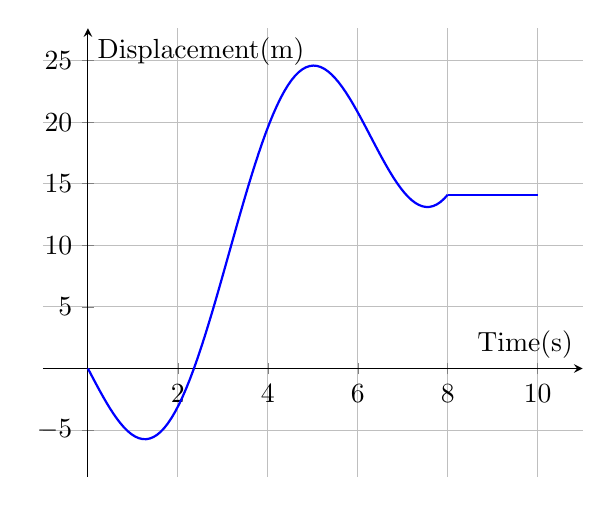
\begin{tikzpicture}
            \begin{axis}[axis lines= middle, xlabel = {Time(s)}, ylabel = {Displacement(m)}, samples = 100, domain= 0:10, enlargelimits = true, xtick = {0,2,4,6,8,10},ytick={-10,-5,0,5,10,15,20,25,30},grid=major]
                \addplot[blue,thick, domain=0:8] {3*x - 10*sin(deg(x))};
                \addplot[blue,thick,domain=8:10] {14.10642};
            \end{axis}
        \end{tikzpicture}
    \end{figure}
\end{center}
{The gradient of the graph is the velocity of the particle, as velocity is given by $\frac{dx}{dt}$. This time if $\frac{dx}{dt}=0$, the particle is stationary in 1D or in orbit in 2D, 3D, 4D, $\ldots$. The area under the graph is nothing particularly useful, but is the absement of the particle.}

\end{document}